\section{Theoretische Grundlagen}
Eine Regelung besteht, wie in Abbildung \ref{regelstrecke} zu sehen ist, aus einem Regler und einer Regelstrecke. Beispiele einer Regelung sind Heizungen oder Geschwindigkeitsregelungen.\newline 

\begin{figure}[h]
\centering
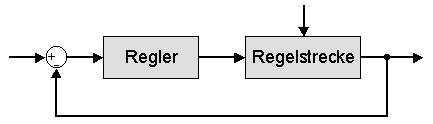
\includegraphics[width=0.8\textwidth]{Regelstrecke.png}
\caption{Regelung bestehend aus Regler und Regelstrecke}
\label{regelstrecke}
\end{figure}
%Quelle: http://rn-wissen.de/wiki/index.php/Datei:Regelkreis4.png [Abrufdatum 6.5.15]


Ist eine Regelstrecke gegeben, im Falle eines Lötkolbens wäre dies die Distanz vom Heizelement bis zur Lötspitze, so muss ein dazu passender Regler dimensioniert werden. Reglerdimensionierungen können über das Auswerten der Schrittantwort der Regelstrecke durchgeführt werden. Um die Schrittantwort zu erhalten wird das Verhalten der Strecke aufgrund eines Schrittes der Eingangsgrösse gemessen. Für die Berechnungen werden die aus der Schrittantwort der Strecke ausgelesenen Kenngrössen Verzugszeit ($T_u$), Anstiegszeit ($T_g$) und Streckenbeiwert ($K_s$) verwendet. Zur Dimensionierung eines passenden Reglers existieren verschiedenste Methoden. Im Folgenden werden nun zwei Möglichkeiten genauer erläutert, wobei das Hauptaugenmerk auf der ersten Methode, der Phasengangmethode, liegt und die zweite, die Dimensionierung mittels gängigen Faustformeln, lediglich zum Vergleich durchgeführt wird.\newline

\newpage
Die Kurve in Abbildung \ref{schrittantwort} stellt die Schrittantwort einer Regelstrecke dar. Daran angelegt ist die Wendetangente, die benötigt wird, um die Verzugs- und die Anstiegszeit messen zu können.\newline

\begin{figure}[h]
\centering
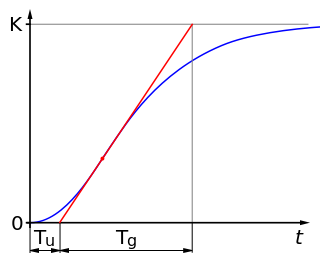
\includegraphics[width=0.6\textwidth]{Schrittantwort.png}
\caption{Schrittantwort einer Regelstrecke}
\label{schrittantwort}
\end{figure}
%Quelle: http://de.wikipedia.org/wiki/Faustformelverfahren_%28Automatisierungstechnik%29#/media/File:Tutg.svg [Abrufdatum 6.5.15]

Ziel ist es, PI- sowie PID-Regler zu dimensionieren, das heisst deren Kennwerte zu berechnen. Der PI-Regler hat die Kennwerte Nachstellzeit ($T_n$) und Reglerverstärkung ($K_R$), beim PID-Regler kommt noch die Vorhaltezeit ($T_v$) hinzu.



\subsection{Streckenanalyse}
Die Streckenidentifikation wird mittels der Sani-Methode durchgeführt. Aus dem Verhältnis von $T_u$ und $T_g$ werden die Ordnung der Strecke und die dazugehörigen Zeitkonstanten berechnet, die benötigt werden, um die Übertragungsfunktion der Regelstrecke darzustellen. \newline 


% Quelle Skript "Mathematisches Labor mlab", Soenicki/Bürgi
Die Übertragungsfunktion der Strecke ist gemäss Formel \ref{ufunkstr} definiert:

\begin{align}
G_S(s)=\frac{K_S}{(1+sT_1)(1+sT_2)...(1+sT_n)}
\label{ufunkstr}
\end{align}

\newpage
\subsection{Phasengangmethode}
Bei der Phasengangmethode handelt es sich eigentlich um eine grafische Dimensionierungsmethode, welche früher noch von Hand mit logarithmischem Papier durchgeführt wurde. Anstelle der grafischen Dimensionierung wird die Methode in diesem Fall komplett rechnerisch gelöst. Um die Methode zu verstehen wird ein theoretisches Grundwissen benötigt, welches in folgenden Unterkapiteln erklärt wird.


\subsubsection{Grundlagen}
Durch Ersetzen von $s$ durch $j\omega$ in der Übertragungsfunktion der Strecke erhält man den Frequenzgang. Um die Phasengangmethode anwenden zu können, wird der Amplituden- und Phasengang der Regelstrecke benötigt.
% Vielleicht noch ein Satz zur Definition a-gang ph-gang, wie man auf die Formeln kommt


\begin{align}
A_S(\omega)=abs(G_S(j\omega))
\end{align}
\begin{align}
\varphi_S(\omega)=arg(G_S(j\omega))
\end{align}
\begin{align}
\varphi_S(\omega)=-arctan(\omega T_1)-arctan(\omega T_2)...-arctan(\omega T_n)
\end{align}\newline

Die Zeitkonstanten des zu dimensionierenden Reglers stehen in direktem Zusammenhang mit dessen Amplitudengang. In den Abbildungen \ref{agangpi} und \ref{agangpid} sind die Amplitudengänge eines PI- und eines PID-Reglers dargestellt, wobei die x-Achsen logarithmisch skaliert sind. Wie die Kreisfrequenzen an den Knickstellen mit den Reglerparametern zusammenhängen sollen, ist in Tabelle \ref{amplitudengaenge} ersichtlich.\newline

\begin{figure}[h]
\centering
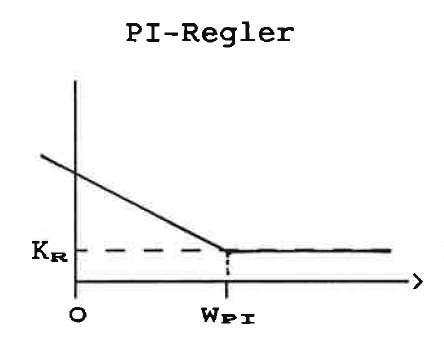
\includegraphics[width=0.5\textwidth]{agangpi.png}
\caption{Amplitudengang PI-Regler Amp($\omega$) (log. Darstellung)}
\label{agangpi}
\end{figure}
%Quelle: Zellwegerskript

\begin{figure}[h]
\centering
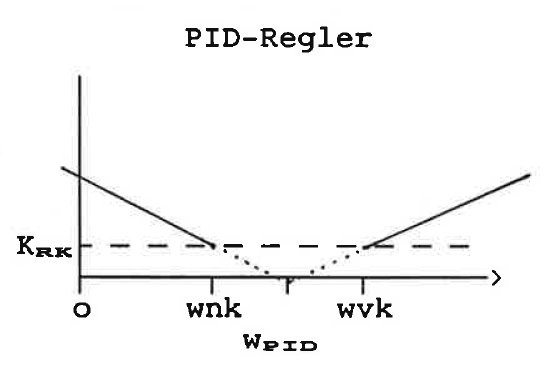
\includegraphics[width=0.6\textwidth]{agangpid.png}
\caption{Amplitudengang PID-Regler Amp($\omega$) (log. Darstellung)}
\label{agangpid}
\end{figure}
%Quelle: Zellwegerskript

\begin{table}[h]
\centering
\renewcommand*{\arraystretch}{1.7}
\begin{tabular}{|l|l|c|}
\hline 
\textbf{PI-Regler} & \multicolumn{2}{c|}{\textbf{PID-Regler}} \\ 
\hline 
$\omega_{PI}=\frac{1}{T_n}$ & $\omega_{nk}=\frac{1}{T_{nk}}=\beta*\omega_{PID}$ & $\omega_{vk}=\frac{1}{T_{vk}}=\frac{\omega_{PID}}{\beta}$ \\ 
\hline 
\end{tabular}
\caption[Amplitudengänge / Knickkreisfrequenzen]{Amplitudengänge Regler und Zusammenhänge mit Knickkreisfrequenzen}
\label{amplitudengaenge}
\renewcommand*{\arraystretch}{1} 
\end{table}

\newpage
Diese Knickkreisfrequenzen werden mithilfe des Phasengangs der Strecke berechnet. Je nach dem welcher Reglertyp dimensioniert werden soll, müssen andere Punkte im Phasengang gesucht werden (Tabelle \ref{phgangpunkte}).\newline

\begin{table}[h]
\centering
\renewcommand*{\arraystretch}{1.7}
\begin{tabular}{|l|c|c|}
\hline 
\textbf{Regler} & \textbf{Phasengang der Strecke $\varphi_s$} & \textbf{Knickkreisfrequenz}  \\ 
\hline 
\textbf{PI} & $-\frac{\pi}{2}=-90^\circ$ & $\omega_{PI}=\frac{1}{T_n}$ \\ 
\hline 
\textbf{PID} & $-\frac{3\pi}{4}=-135^\circ$ & $\omega_{PID}=\frac{1}{\sqrt{T_{nk}T_{vk}}}$ \\ 
\hline 
\end{tabular}
\caption[Wichtige Phasengangpunkte]{Gesuchte Punkte im Phasengang je nach Regler}
\label{phgangpunkte}
\renewcommand*{\arraystretch}{1} 
\end{table}

\newpage
Der PI-Regler kann anhand dieser Dimensionierungskriterien bereits dimensioniert werden. Beim PID-Regler muss allerdings noch ein Parameter mehr bestimmt werden. Es handelt sich um den Faktor $\beta$ welcher benötigt wird um die Knickkreisfrequenzen des PID-Reglers berechnen zu können. Dieser Faktor $\beta$ hängt mit der Tangentensteigung des Phasengangs der offenen Regelung im Punkt $-135^\circ$ zusammen.\newline
Ein Dimensionierungskriterium der Phasengangmethode lautet, dass die Steigung des Phasengangs der gesamten, offenen Regelung bei der Knickkreisfrequenz $\frac{-0.5}{\omega_{PID}}$ betragen soll. Dies hat damit zu tun, dass eine Steigung von -20dB/Dekade angestrebt wird. Die genaue Herleitung von $\beta$ befindet sich im Anhang. \newline

Es gilt also die folgende Beziehung:\newline

\begin{align}
\frac{2\beta}{1+\beta^2} + \omega_{PID}\frac{d\varphi_{Strecke(\omega_{PID})}}{d\omega} = -0.5
\end{align}\newline

Da der Phasengang der Strecke und somit dessen Ableitung gegeben ist, kann durch Auflösen nach $\beta$ nun auch dieser Parameter ermittelt werden. Ergibt sich ein Wert grösser als eins oder imaginär, so wird $\beta$ als eins angenommen.

Die Verstärkung des Reglers wird mit Hilfe des Phasenrands bestimmt. Der Phasenrand ist die Differenz der Streckenphase zu $-180^\circ$. Bei unterschiedlichem Phasenrand ergeben sich unterschiedliche Verstärkungsfaktoren, was auch auf das Überschwingen des Reglers Einfluss hat. Tabelle \ref{phasenrand} zeigt den Zusammenhang zwischen dem gewählten Phasenrand und dem daraus resultierenden Überschwingen der Regelung.\newline


\begin{table}[h]
\centering
\renewcommand*{\arraystretch}{1.2}
\begin{tabular}{|c|c|c|}
\hline 
\textbf{Phasenrand $\varphi_R$} & \textbf{Streckenphase $\varphi_S$} & \textbf{Überschwingen} \\ 
\hline 
$45^\circ$ & $-135^\circ$ & $23\%$ \\ 
\hline 
$51.8^\circ$ & $-128.5^\circ$ & $16.3\%$ \\ 
\hline 
 $65.5^\circ$& $-114.6^\circ$ & $4.6\%$ \\ 
\hline 
$76.3^\circ$ & $-103.7^\circ$ & $0\%$ \\ 
\hline
\end{tabular} 
\caption{Zusammenhang Phasenrand und Überschwingen}
\label{phasenrand}
\renewcommand*{\arraystretch}{1}
\end{table}

\newpage
Zur Berechnung der Verstärkung werden nun die Amplitudengänge der Strecke, sowie des Reglers benötigt. Die Werte dieser beiden Amplitudengänge an der Stelle wo der Phasenrand abgetragen wurde, werden miteinander multipliziert. Gemäss Phasengangmethode soll die Verstärkung an dieser Stelle eins sein. Dies führt zur Formel \ref{formelkr}:\newline
\begin{align}
K_R=\frac{1}{\vert{Go(\omega_D)}\vert{}}
\label{formelkr}
\end{align}


\subsubsection{Ablauf der Phasengangmethode}
Die Phasengangmethode der Strecke $\varphi_S$ wird nach dem folgenden Ablauf durchgeführt. Die Punkte 2. und 3. werden nur für PID-Regler benötigt. Eine numerische Beispielrechnung für einen PI-Regler ist im Anhang angefügt.
\begin{enumerate}
\item Im Phasengang der Strecke $\varphi_S$ werden die Kreisfrequenzen in bestimmten Punkten gesucht.
\item Der Faktor $\beta$ wird bestimmt.
\item Mithilfe von $\beta$ werden die Zeiten $T_{nk}$ und $T_{vk}$ ermittelt.
\item Der Phasengang der offenen Regelung $\varphi_{go}$ wird berechnet (Phasengang Strecke + Phasengang Regler)
\item Die Kreisfrequenz $\omega_D$ beim gewählten Phasenrand wird berechnet.
\item Die Amplitudengänge der Strecke sowie des Reglers bei $\omega_D$ werden miteinander multipliziert. Damit wird die Reglerverstärkung $K_R$ festgelegt. 
\end{enumerate}

Besondere Vorsicht ist bei den erhaltenen Kenngrössen des dimensionierten Reglers geboten. Es wird zwischen Regler- und Bodekonform unterschieden. Bodekonform bedeutet, dass die Parameter kaskadiert sind und die logarithmische Rechnung somit vereinfacht wird. Standardmässig wird in der Fachliteratur meist reglerkonform gerechnet. Die Parameter des PI-Reglers sind reglerkonform und können somit direkt weiterverwendet werden. Die Parameter des PID-Reglers, welche wir bei der Dimensionierung mittels Phasengangmethode erhalten, sind bodekonform. Sie können jedoch in die reglerkonforme Darstellung umgerechnet werden. Für die Umrechnung wurden die Formeln \ref{krherl}, \ref{tnherl} und \ref{tvherl} für PID-Regler hergeleitet (siehe Anhang): \newline


\begin{align}
K_R=K_{rk}\left(1+\frac{T_{vk}}{T_{nk}}-\frac{T_p}{T_{nk}}\right)
\label{krherl}
\end{align}
\begin{align}
T_n=T_{nk}+T_{vk}-T_p
\label{tnherl}
\end{align}
\begin{align}
T_v=\frac{T_{nk}T_{vk}}{T_{nk}+T_{vk}-T_p}-T_p
\label{tvherl}
\end{align}\newline

Tp steht für die parasitäre Zeitkonstante. Diese wird benötigt, da ein idealer PID-Regler in der Praxis nicht umsetzbar ist. Der Index k in der bodekonformen Darstellung steht für Kaskadierung.

\subsection{Übertragungsfunktion der Regler}
Um schlussendlich die Schrittantwort der geschlossenen Regelung berechnen zu können, wird die Übertragungsfunktion des dimensionierten Reglers benötigt. Diese lässt sich mit den aus der Phasengangmethode erhaltenen Parametern aufstellen (Tabelle \ref{ufunkregler}).\newline
\begin{table}
\centering
\renewcommand*{\arraystretch}{1.7}
\begin{tabular}{|l|l|}
\hline 
\textbf{Beschreibung} & \textbf{Darstellung} \\ 
\hline
PI-Regler bodekonform & $G_R(s)=K_R\frac{(1+sT_n)}{sT_n}$ \\ 
\hline 
PI-Regler reglerkonform & $G_R(s)=K_R\left(1+\frac{1}{sT_n}\right)$ \\ 
\hline 
PID-Regler bodekonform & $G_R(s)=K_{rk}\frac{(1+sT_{nk})(1+sT_{vk})}{sT_{nk}(1+sT_p)}$ \\ 
\hline 
PID-Regler reglerkonform & $G_R(s)=K_R\left(1+\frac{1}{sT_n}+\frac{sT_v}{1+sT_p}\right)$ \\ 
\hline 
\end{tabular} 
\renewcommand*{\arraystretch}{1}
\caption{Übertragungsfunktionen Regler}
\label{ufunkregler}
\end{table}

\newpage
\subsection{Dimensionierung mit Faustformeln}
Die Dimensionierung mittels Faustformeln wird durchgeführt, um die Dimensionierungsresultate der Phasengangmethode am Schluss zu vergleichen und auszuwerten. Es gibt etliche verschiedene Faustformeln von unterschiedlichen Personen. Die bekanntesten und gängigsten Dimensionierungsformeln sind in den folgenden Tabellen aufgelistet und werden im Programm implementiert.\\

\begin{table}[h]
\centering
\renewcommand*{\arraystretch}{1.7}
\begin{tabular}{|l|c|c|c|}
\hline 
\textbf{Regler} & \textbf{$K_R$} & \textbf{$T_n$} & \textbf{$T_v$} \\ 
\hline 
\textbf{P} & $\frac{T_g}{K_sT_u}$ &  &  \\ 
\hline 
\textbf{PI} & $\frac{0.9*T_g}{K_sT_u}$ & $3.3*T_u$ &  \\ 
\hline 
\textbf{PID} & $\frac{0.9*T_g}{K_sT_u}$ & $2*T_u$ & $0.42*T_t$ \\ 
\hline 
\end{tabular} 
\renewcommand*{\arraystretch}{1}
\caption{Ziegler/Nichols}
\end{table}

\begin{table}[h]
\centering
\renewcommand*{\arraystretch}{1.7}
\begin{tabular}{|l|c|c|c|}
\hline 
\textbf{Regler} & \textbf{$K_R$} & \textbf{$T_n$} & \textbf{$T_v$} \\ 
\hline 
\textbf{P} & $\frac{T_g}{K_sT_u}$ &  &  \\ 
\hline 
\textbf{PI} & $\frac{0.8*T_g}{K_sT_u}$ & $3*T_u$ &  \\ 
\hline 
\textbf{PID} & $\frac{1.2*T_g}{K_sT_u}$ & $2*T_u$ & $0.42*T_t$ \\ 
\hline 
\end{tabular} 
\renewcommand*{\arraystretch}{1}
\caption{Oppelt}
\end{table}

\begin{table}[h]
\centering
\renewcommand*{\arraystretch}{1.7}
\begin{tabular}{|l|c|c|c|}
\hline 
\textbf{Regler} & \textbf{$K_R$} & \textbf{$T_n$} & \textbf{$T_v$} \\ 
\hline 
\textbf{P} & $\frac{T_g}{K_sT_u}$ &  &  \\ 
\hline 
\textbf{PI} & $\frac{0.91*T_g}{K_sT_u}$ & $3.3*T_u$ &  \\ 
\hline 
\textbf{PID} & $\frac{1.2*T_g}{K_sT_u}$ & $2*T_u$ & $0.44*T_t$ \\ 
\hline 
\end{tabular} 
\renewcommand*{\arraystretch}{1}
\caption{Rosenberg}
\end{table}

\begin{table}
\centering
\renewcommand*{\arraystretch}{1.5}
\begin{tabular}{|l|c|c|c|c|}
\hline 
& \multicolumn{2}{c|}{\textbf{aperiodischer}} & \multicolumn{2}{c|}{\textbf{Einschwingvorgang mit}} \\
\textbf{Reglertyp} & \multicolumn{2}{c|}{\textbf{Einschwingvorgang}} & \multicolumn{2}{c|}{\textbf{20\% Überschwingen}}\\
\cline{2-5} 
 & Führung & Störung & Führung & Störung \\ 
\hline 
\textbf{P} & $K_R=\frac{0.3*T_g}{K_sT_u}$ & $K_R=\frac{0.3*T_g}{K_sT_u}$ & $K_R=\frac{0.7*T_g}{K_sT_u}$ & $K_R=\frac{0.7*T_g}{K_sT_u}$ \\ 
\hline 
\multirow{2}{*}{\textbf{PI}} & $K_R=\frac{0.35*T_g}{K_sT_u}$ & $K_R=\frac{0.6*T_g}{K_sT_u}$ & $K_R=\frac{0.6*T_g}{K_sT_u}$ & $K_R=\frac{0.7*T_g}{K_sT_u}$ \\ 
& $T_n=1.2*T_g$ & $T_n=4*T_u$ & $T_n=T_g$ & $T_n=2.3*T_u$ \\ 
\hline 
 & $K_R=\frac{0.6*T_g}{K_sT_u}$ & $K_R=\frac{0.95*T_g}{K_sT_u}$ & $K_R=\frac{0.95*T_g}{K_sT_u}$ & $K_R=\frac{1.2*T_g}{K_sT_u}$\\ 
\textbf{PID} & $T_n=T_g$ & $T_n=2.4*T_u$ &  $T_n=1.35*T_g$ & $T_n=2.3*T_u$ \\ 
 & $T_v=0.5*T_u$ & $T_v=0.42*T_u$ & $T_v=0.47*T_u$ & $T_v=0.42*T_u$ \\ 
\hline 
\end{tabular}
\renewcommand*{\arraystretch}{1}
\caption{Chien/Hrones und Reswick} 
\end{table}


\newpage
\subsection{Schrittantwort der Regelung}
- Übertragungsfunktion Regelung (Berechnung aus üfunk regler und üfunk regelung)\newline
- Berechnung durch Residuen\newline

Um die Schrittantwort der geschlossenen Regelung berechnen zu können, wird die Übertragungsfunktion der Regelung benötigt. Diese wird aus den Übertragungsfunktionen des Reglers und der Strecke gemässe Formel \ref{ufunkregelung} berechnet.

\begin{align}
G(s)=\frac{G_R(s)G_S(s)}{1+G_R(s)G_S(s)}
\label{ufunkregelung}
\end{align}
